\documentclass[11pt,letterpaper]{article}
%\documentclass[11pt,letterpaper]{exam}
\usepackage[latin1]{inputenc}
\usepackage[left=3.00cm, right=3.00cm, top=3.00cm, bottom=3.00cm]{geometry}

\usepackage{amsmath}
%\usepackage{amsthm}
%\usepackage{cancel}
\usepackage{mathtools}
%\DeclarePairedDelimiter\ceil{\lceil}{\rceil}
%\DeclarePairedDelimiter\floor{\lfloor}{\rfloor}

\usepackage{fancyhdr}
\pagestyle{fancy}

\usepackage{color}
%\usepackage{xcolor}
%\usepackage{graphicx}
\usepackage{caption}
%\definecolor{acolour}{rgb}{0,0.0,0}

%\usepackage{url}
\usepackage{listings}
%\usepackage[]{algorithm2e}

\lstset{frame=tb,
	language=Java,
	aboveskip=3mm,
	belowskip=3mm,
	showstringspaces=false,
	%frame=tb,
	columns=flexible,
	basicstyle={\small\ttfamily},
	numbers=none,
	numberstyle=\tiny\color{gray},
	keywordstyle=\color{blue},
	commentstyle=\color{dkgreen},
	stringstyle=\color{mauve},
	breaklines=true,
	breakatwhitespace=true,
	tabsize=3
}

\newcounter{nalg}[section] % defines algorithm counter for chapter-level
\renewcommand{\thenalg}{\thechapter .\arabic{nalg}} %defines appearance of the algorithm counter
\DeclareCaptionLabelFormat{algocaption}{Algorithm \thenalg} % defines a new caption label as Algorithm x.y

\lstnewenvironment{algorithm}[1][] %defines the algorithm listing environment
{   
	\refstepcounter{nalg} %increments algorithm number
	\captionsetup{labelformat=algocaption,labelsep=colon} %defines the caption setup for: it uses label format as the declared caption label above and makes label and caption text to be separated by a ':'
	\lstset{ %this is the stype
		mathescape=true,
		frame=tB,
		numbers=left, 
		numberstyle=\tiny,
		basicstyle=\scriptsize, 
		keywordstyle=\color{blue}\bfseries\em,
		keywords={,input, output, return, datatype, function, in, if, else, foreach, while, begin, end, true, false, int, for, then, } %add the keywords you want, or load a language as Rubens explains in his comment above.
		numbers=left,
		xleftmargin=.02\textwidth,
		#1 % this is to add specific settings to an usage of this environment (for instnce, the caption and referable label)
	}
}
{}

\author{Simon Zheng\\260744353}
\title{Homework 1}
\date{January 30$^{\textnormal{th}}$, 2018}
\lhead{COMP 424}
%\chead{Homework $$}
\rhead{Artificial Intelligence}

\begin{document}
	\maketitle
	\thispagestyle{fancy}
	
	\section{Six-Puzzle}
		\subsection{a)}
		\begin{figure}[ht]
			\centering
			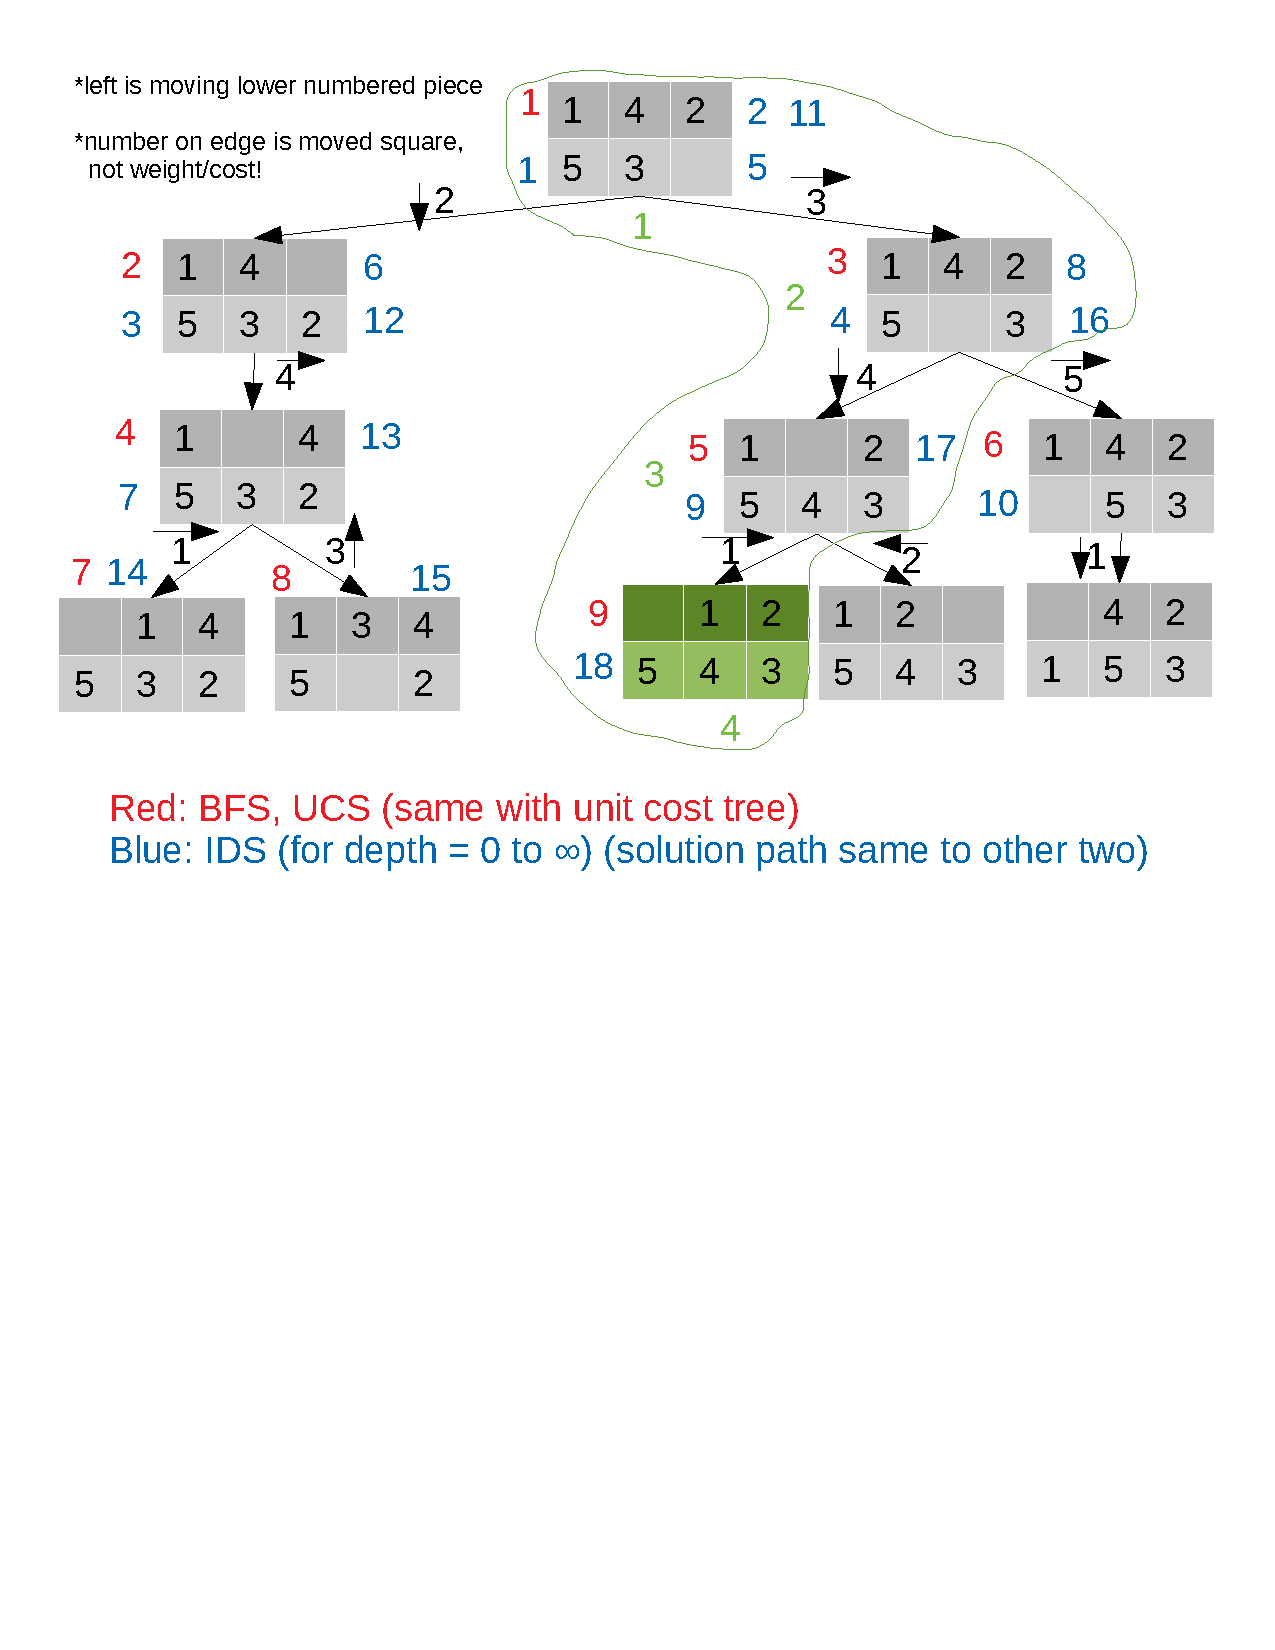
\includegraphics[height=300px,width=400px,trim={0 360px 0 0},clip]{q1.pdf}
			\linespread{0.8}\caption{Search tree}
		\end{figure}
		
		\subsection{b)}
		Yes.
		If we use Manhattan distance, then we have an underestimating (optimistic) heuristic as it is exactly calculating the most direct path from a square's current position to its goal position.
		In a version of the puzzle where squares can move over each other, it is optimal.
		
		If we add cost (based on square values), we are not changing this fact, as while the cost would increase, Manhattan would still be the same most optimistic path so the smallest (unit) cost.
		
		\subsection{c)}
		In this case, we simply use a sort of "Manhattan distance" except each movement has a cost of its value (multiply the distance for each square as the final cost) for the heuristic.
		
		It is still optimistic for the same reason as previously explained, but with the cost factored in the calculations, it dominates the unit cost version.
		
		\subsection{d)}
		No.
		Manhattan distance would overestimate every up and down movement.
		It would still be optimistic for most cases (as there are only two rows so at most one up and down movement but one or two left and right movement) but for the simple case of the distance being one and so only moving once up or down, Manhattan would estimate 1 even though the cost is 0.5.
		
	\section{Search algorithms}
	    \subsection{a)}
	    A state space which is a tree with a single branch, where each child has a single child (a path) is $O(n)$ for DFS (just go down the tree) but $\sum_{k=1}^{n} = O(n^2)$ for IDS as it keeps restarting at every depth.
	    
	    \subsection{b)}
	    True.
	    If you run UCS on a graph with unit costs (or equal costs), then it will behave like BFS, thus BFS is a special case of UCS with unit costs.
	    The algorithm would not prioritize one child or neighbor over another since the cost is not better or worst for any of them.
	    Instead, the depth would add up equally and thus this UCS would expand the lowest depth nodes first.
	    Thus, the priority queue acts as a normal queue and the algorithm behave as a BFS.
	    
	    \subsection{c)}
	    True.
	    A Best-First Search which uses a heuristic function where it expands the deepest node first behaves like DFS.
	    The heuristic would evaluate the negative depth (from the root node) such that a larger depth has an inferior cost.
	    
	    \subsection{d)}
	    True.
	    We know that an A* Search evaluates which nodes to expand based on a function which calculates the cost and uses a heuristic.
	    As an uninformed search, UCS would simply ignore the heuristic part of the evaluation function.
	    Thus, what we are left with is the cost function, which would simply be a UCS.
	
	\section{Optimization}
	
	\section{Constraint satisfaction}
	    \subsection{a)}
	    \begin{itemize}
            \item Variables: rooks $\{R_1, R_2, ... , R_k\}$ (one rook per row which is the index, value is column)
            \item Domain: $\{1, 2, ... , n\}$, $k \in \mathbf{N}$
            \item Constraints: $k \leq n^2$ or $k \le $ $R_i \neq R_j$ (no two rooks can be on the same column)
        \end{itemize}
        
        \subsection{b)}
        \begin{figure}[ht]
			\centering
			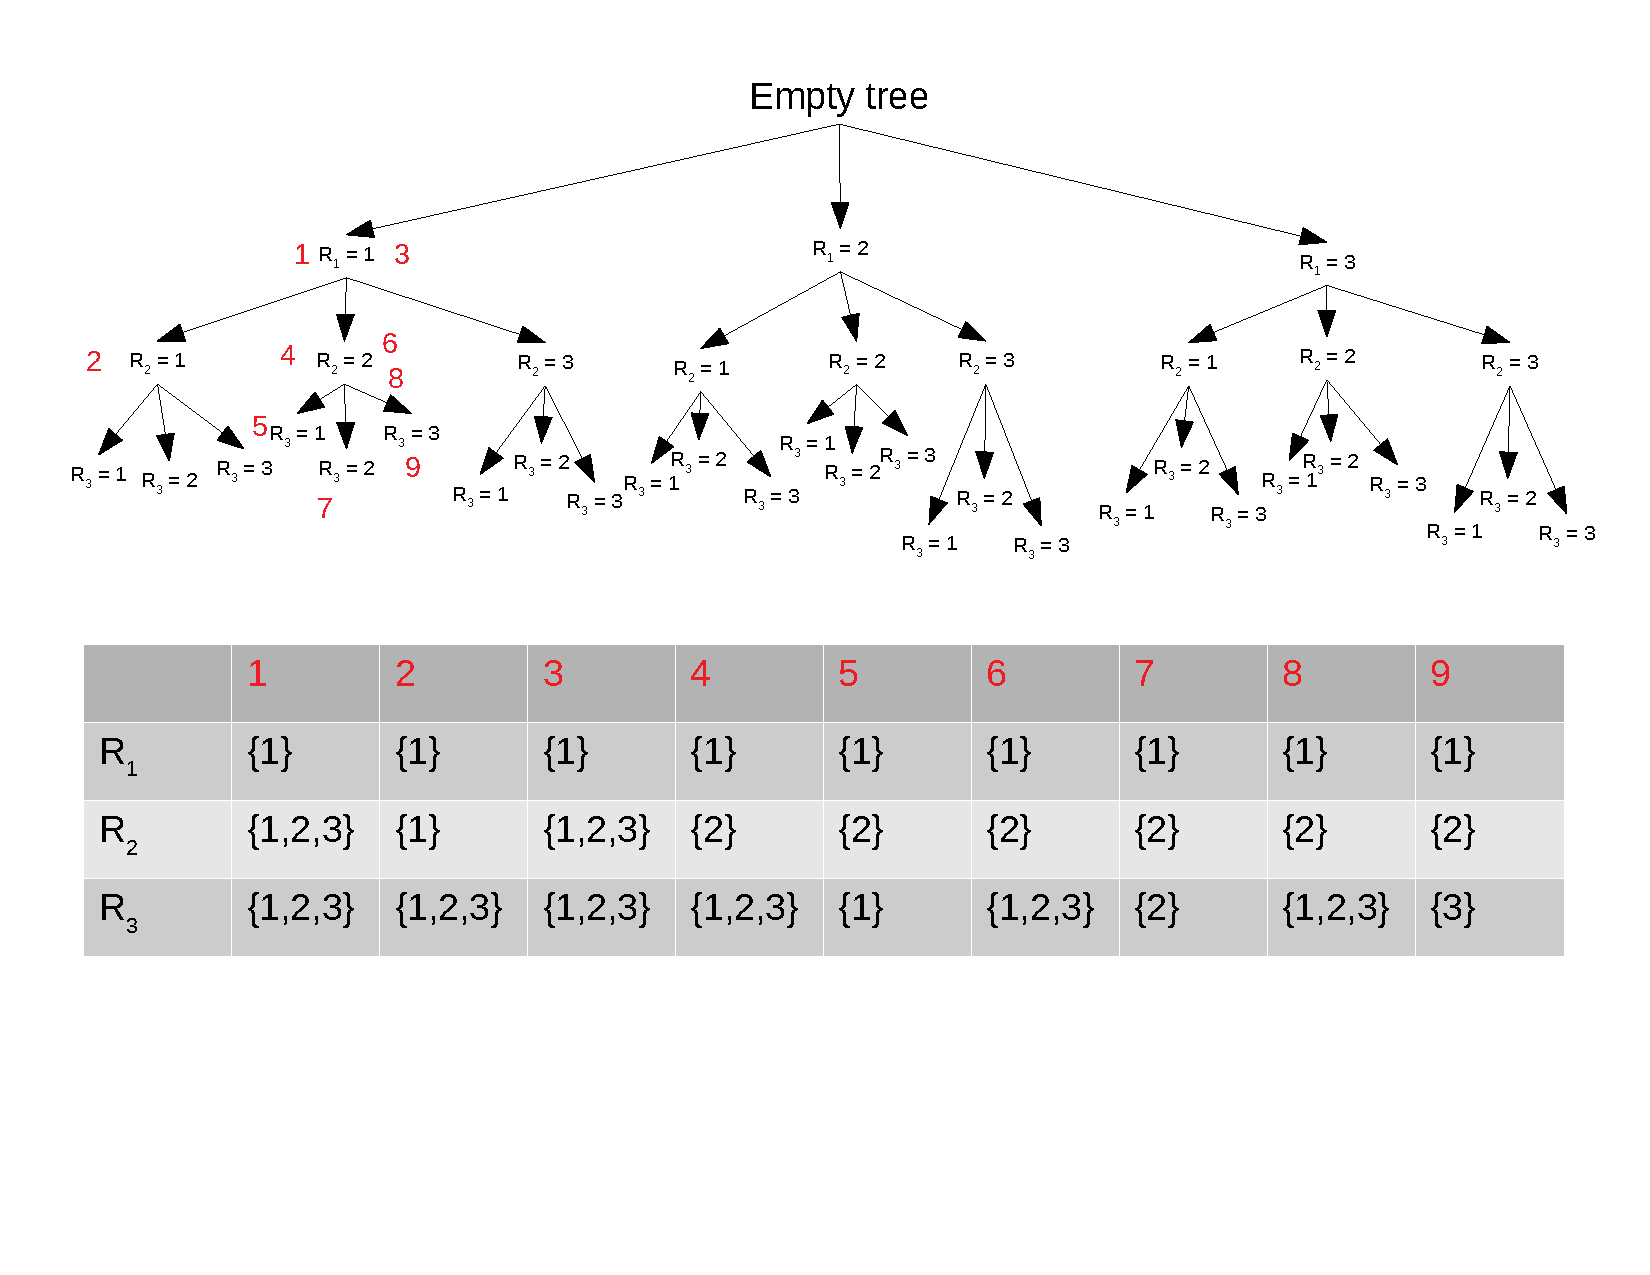
\includegraphics[height=250px,width=425px,trim={0 150 0 0},clip]{q4.pdf}
			\linespread{0.8}\caption{Search tree without forward checking. The backtracking algorithm would only generate the nodes marked with red numbers.}
		\end{figure}
        
        \subsection{c)}
        \begin{figure}[ht]
			\centering
			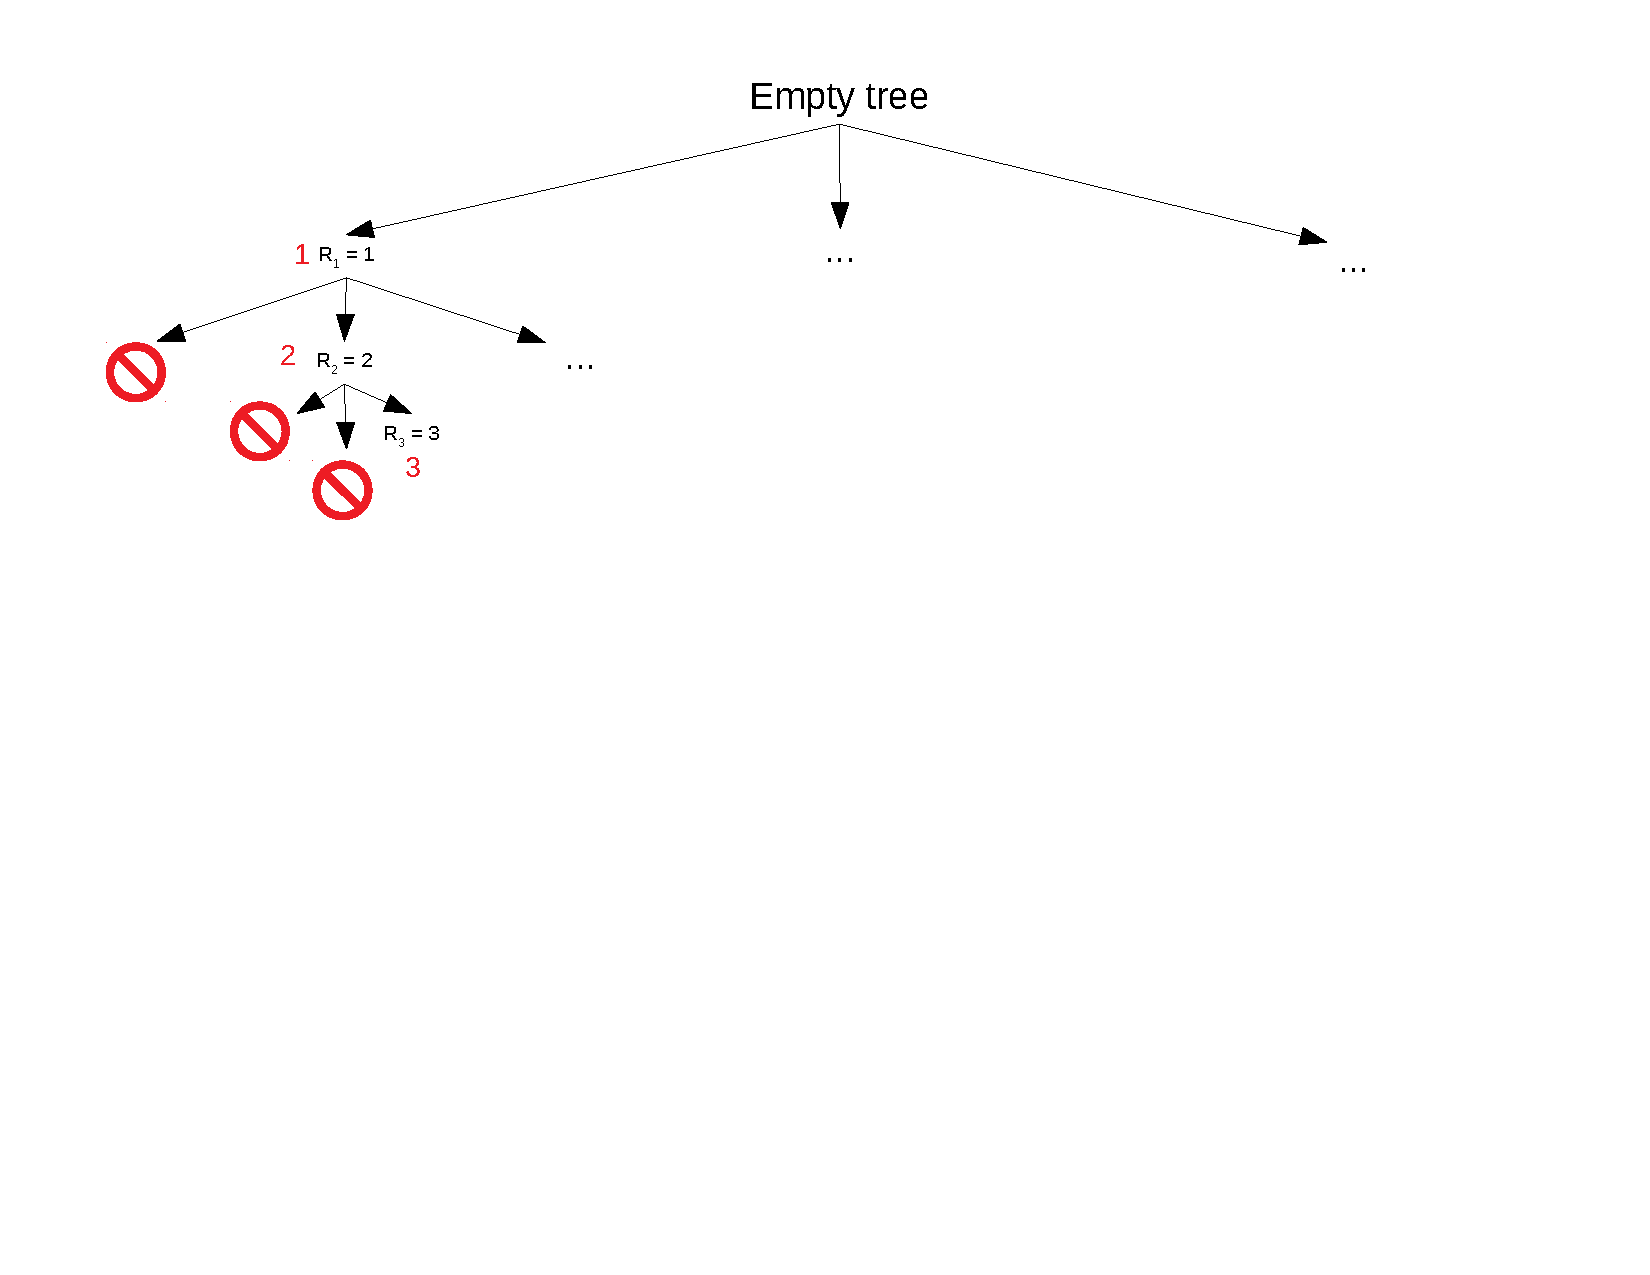
\includegraphics[height=175px,width=425px,trim={0 350 100 0},clip]{q4c.pdf}
			\linespread{0.8}\caption{Search tree with forward checking.}
		\end{figure}
	
\end{document}
